\label{sec:background}
%Before diving into the description of our contributions, we introduce the fundamental background of our work.

In multicore settings, assessement of the execution time and memory interference has become a challenge because the number of possible interleavings increases exponentially with the number of processes, number of cores and number of shared resources \cite{Chatto2012}. In practice, concurrent programs may have astronomical numbers of legal interleavings which makes the interleaving analysis not feasible. An alternative is to reuse the knowledge acquired from the single core analysis and just focus on the interference resulting from the access to shared memories. This section introduces benchmarking, as a technique to measure WCET and WCRA, as well as the fundamental background of our work.

\begin{figure}[ht!]
\centering
\caption{Simplified multicore system architecture.}
\label{fig:architecture}
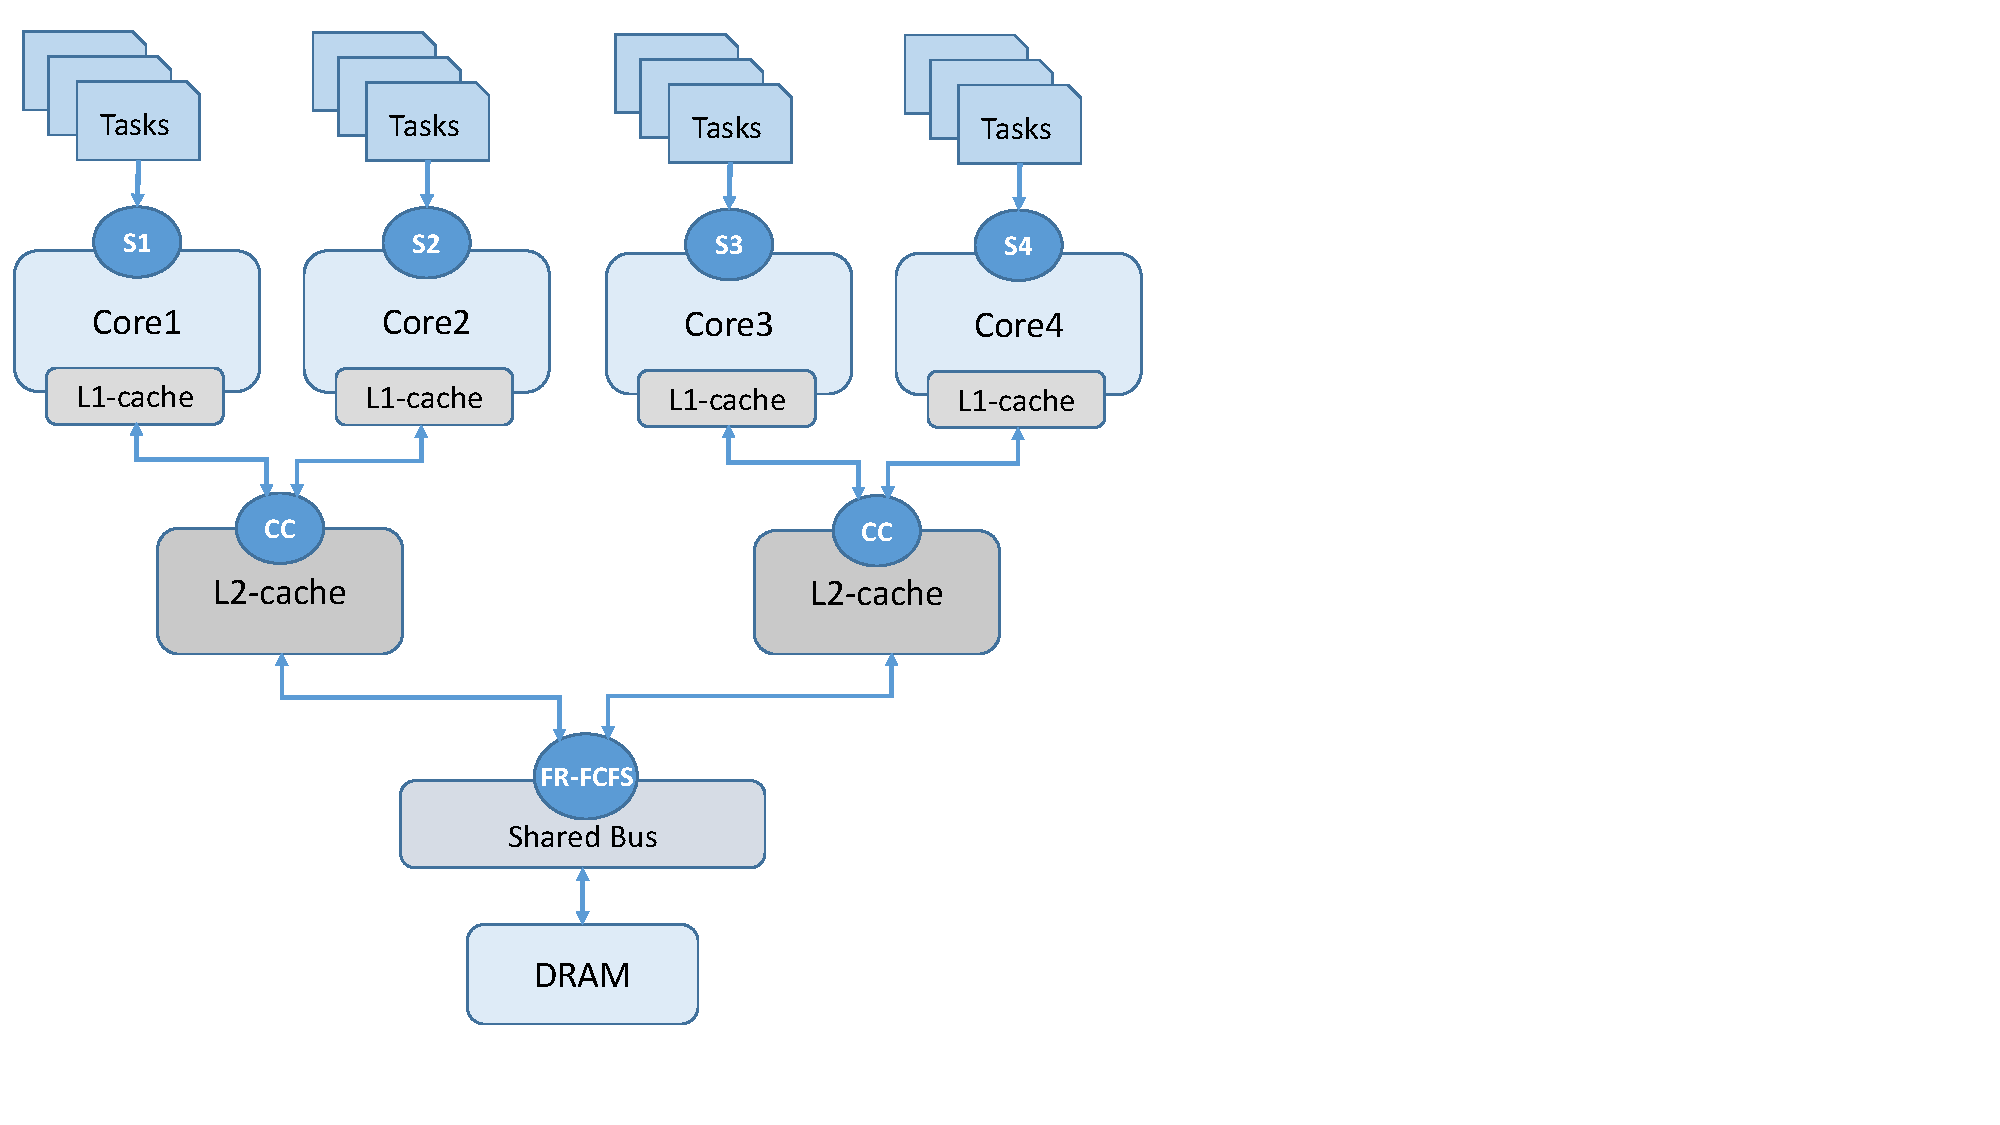
\includegraphics[scale=0.45]{architecture.pdf}
\end{figure}

The overall system architecture we consider in this paper is depicted in Fig.~\ref{fig:architecture}, where $cc$ is the cache coloring policy and $s_i$ are CPU scheduling policies.

\subsection{Systems Benchmarking} 
\label{sec:methodology}
Throughout this section we describe how the inputs required by our model-based framework are obtained form an actual system, in particular WCETs and WCRAs. In software engineering, benchmarking \cite{Benchmarking} aims at measuring a set of execution attributes and performance characteristics, e.g. WCET, of a given software system. %The user has to run the application to be benchmarked on the target platform to determine for example the execution time of each process. 
The output of a system benchmarking (shortly known by benchmark) will be used to reconstruct a behavioral model of the system,  which can be used in turn for simulation and analysis purposes. Benchmarking is known as an expensive operation that involves several iterative rounds in order to reach conclusive decisions. %In this context, we are interested in how WCET and WCRA are derived from a concrete multicore software system. 
Roughly speaking, flow analysis and profiling are the most commonly used techniques to measure the WCET and WCRA of application tasks.  

Flow analysis \cite{Tan2009,Chatto2012} is a technique to estimate the WCET of a program. It consists of simulating, or concretely running, a program in isolation and measuring the time spent. Technically, static analysis tools use symbolic execution engines to identify potential execution paths without necessarily having to run the program. Such representations can be structured in terms of control flow graph (CFG). %Similarly to compilers, a static analysis tool parses a source code of a program and converts it to an intermediate representation where each state could be a class of different program configurations. 
WCET is then the time spent when executing the longest path of the CFG. Static analysis has been practiced for the analysis of software systems via different analysis tools, e.g. {SWEET} \cite{Tan2009}. 
%The depth of the model determines the effectiveness of the tool. That depth is based on how much knowledge of program behaviour is built in, how much of the program it can take into account at once and how accurately it reflects actual program behaviour. 

%Conventionally, task periods and deadlines (potentially also priority and criticality levels) are identifiable during the requirements analysis.

System profiling \cite{Yun2012,Kim14} is a measurement-based approach to estimate how many times a process accesses  shared memories. The system being analyzed is run for a sufficient number of times, each of which for a long enough duration enabling the execution of most of the system functions (code). The analysis focuses on each process individually, so that for each run we track how many times a process accesses a given shared memory. However, due to technology limitations, the measurements can be performed at core level only, so that the obtained access number of a given core corresponds to the set of processes running on top of it. In order to obtain the memory access number for each process, one needs to run each process individually on one core during the analysis, so that the access number obtained corresponds to the process being run. The number of accesses for each core can be obtained using Performance Monitor Counters (PMCs) \cite{Yun2012}, equipping certain multicore platforms. %Such a number is commonly called \textit{Worst Case Resource Access} (WCRA) \cite{Nowotsch14}. 

In literature \cite{Kim14,Yun2012}, profiling and static analysis techniques are not completely differentiated. Both techniques can be used to measure WCET and WCRA.
  

%Once the attributes of system tasks are determined, one can apply rigourous schedulability analysis tools suing either analytic approaches \cite{***} or model-based enginnering approaches \cite{***}.   
 
\subsection{Core-centric Scheduling}
To leverage the processing performance of a computing system, a processing unit (core in our context) can be assigned more than one task, however only one task can execute effectively at any point in time. The arbitration between the different tasks execution is performed according to a scheduling policy. 

Basically, a scheduling policy determines, at any point in time, which task from the ready queue must execute first and whether a given task should be preempted by another. Such a ready queue can be either local for a given core (Local scheduling) or common for a set of cores (Global Scheduling). The most commonly used scheduling algorithms are {Earliest Deadline First} (EDF), {Fixed Priority Scheduling} (FPS) and {Rate Monotonic} (RM). The key factor in selecting a task from the ready queue can be assigned to the priority, remaining execution time, etc. 
 
In our setting, we adopt FIFO, FPS and EDF as scheduling policies for the individual cores.  %Classic static (cyclic) scheduling used in aerospace contexts can also be coded as a policy if needed. 

\subsection{Memory-centric Scheduling}

%In multicore settings, where different applications running concurrently on different cores compete for the combination of local cache misses and interference delay for accessing a shared  memory can be large and highly variable depending on the platform architecture and the number of parallel access requests. 

With the goal to reduce memory interference in multicore systems, a recent alternative to schedule memory-intensive application tasks is the use of a memory-centric policy \cite{Yao2015,Yao2012}. Tasks assigned to the same core are sorted in the ready queue according to a decreasing order of their WCRA (numbers of memory accesses). 

We distinguish between the access numbers to L2 and DRAM, when comparing 2 tasks we prioritize first the task having more DRAM access requests as DRAM access is more expensive than accessing shared cache L2. If both tasks have the same DRAM access number of requests we refer then to their L2 access number where task having higher number is scheduled first.


 

\subsection{Shared Memory Access Scheduling}
In order to enhance the processing performance of multicore platforms, some of modern multicore processors \footnote{E.g. {Intel Core i7, AMD FX, ARM Cortex and FreeScale QorIQ} processors.} consider a shared cache level (L2-cache) besides to private caches (L1-cache). The primary goal of sharing a cache between different cores is to reduce the access requests to the main memory DRAM  %further, and by that shorten the DRAM interference time since the interference time is strongly correlated to the number of access requests
 \cite{Nowotsch14}. %On the other hand, uncontrolled sharing of cache can lead to a degradation of performance and lack of predictability where starvation can arise. 


Cache coloring policy \cite{Hyoseung13,Ye2014} is an algorithm to control the access to the shared cache level L2. It has been introduced to aid performance optimization where physical memory pages are mapped to cache pages, in contrast with old caching systems where virtual memory is mapped to the cache. This entails avoiding the clearance of cache pages on each context switch. 
During execution, the algorithm frees the old pages as necessary in order to make space for currently scheduled applications (recoloring). The coloring algorithm sorts the concurrent access requests according to their release times.  
 
%Another alternative to schedule accesses to DRAM, in presence of a three-dimensional structure (bank, row and column), is the {Hit-First} policy. The Hit-First algorithm schedules row buffer hits before misses to reduce the average memory access latency and to improve bandwidth utilization \cite{Hong99,Rixner2000}. This is due to the fact that requests hitting in the row buffer have shorter latency than a row buffer miss.

To maximize data throughput and minimize the DRAM latency, DRAM controllers in modern COTS-based systems use {First Ready-First Come First Serve} (FR-FCFS) as a DRAM policy \cite{Rixner2000,Kim14}. FR-FCFS considers a detailed DRAM architecture structured in terms of banks, rows and columns. %The DRAM scheduler can be viewed as a 2-level filter: bank level and bus level. 
The access requests can target different banks separately, where they will be queued in the corresponding bank queue with a special preference to read requests since they cause the processor to stall. % while write requests can normally be performed using write buffers. 
Access requests will be sorted at each bank queue first according to their readiness. Thereafter, the candidates selected from banks level will be further sorted at bus level where the earliest request gains access, i.e. the first request showing up at bus level among the requests being selected by bank schedulers. If no request hits the row-buffer, older requests are prioritized over younger ones.  

In our framework, we do not consider the detailed internal architecture and size of DRAM and shared cache. We focus rather on measuring the delays caused by the concurrent accesses. The reason behind this is that the impact of these characteristics on the
interference is already captured when performing the static analysis and identifying the WCRAs. Hence, estimating the optimal cache size for each application and cache recoloring are beyond the scope of this paper.


\subsection{Statistical Model Checking}
We are using \uppaalsmc \cite{SMC} to perform a formalized statistical simulation of our models, known as Statistical Model Checking (SMC). SMC enables quantitative performance measurements instead of the Boolean (true, false) evaluation that symbolic model checking techniques provide.    
We can summarize the main features of \uppaalsmc in the following:
\begin{itemize}
\item Stopwatches \cite{DBLP:conf/concur/CassezL00} are clocks that can be stopped and resumed without a reset. They are very practical to measure the execution time of preemptive tasks.
\item Simulation and estimation of the expected minimum or maximum value of expressions over a set of runs, \texttt{E[bound](min:expr)} and \texttt{E[bound](max:expr)}, for a given simulation time and/or number of runs specified by \texttt{bound}. 
\item Probability evaluation \texttt{Pr[bound] (P)} for a property \texttt{P} to be satisfied within a given simulation time and/or number of runs specified by \texttt{bound}. \texttt{P} is specified using either LTL or tMITL logic. 
\end{itemize}

Statistical model checking does not provide complete certainty that a property is satisfied, but only verifies it up to a specific confidence level \cite{DBLP:conf/formats/DavidLLMPVW11}, given as an analysis parameter.
